\section{Introduction}
\label{sec:intro}

% \todo{Abhinav and Roger will the introduction}

The last few years have seen a rise in the popularity of Mixture-of-Experts (MoE) based Large Language Models (LLMs)~\citep{deepseekai2025deepseekv3technicalreport,yang2025qwen3technicalreport,5team2025glm45agenticreasoningcoding}. MoEs help LLMs achieve higher accuracy at a lower active parameter count than regular dense models~\citep{dai2024deepseekmoe,lepikhin2020gshard}. Orthogonal to MoEs, Hybrid Mamba-Attention models have shown promise in significantly improving inference throughput~\citep{nemotronnanov2}. We combine these two directions of improvement in Nemotron 3~\citep{nvidia2025nvidianemotron3efficient}. As part of our Nemotron 3 series of models, we present \ourmodel---a 12 billion active, 120 billion total parameter MoE hybrid Mamba-Attention model. \ourmodel achieves better or on-par benchmark accuracies than GPT-OSS-120B~\citep{openai2025gptoss120bgptoss20bmodel} and Qwen3.5-122B while achieving up to 2.2$\times$ and 7.5$\times$ higher inference throughput, respectively, on the 8k token input / 64k token output setting.   %<speed claim> 

\begin{figure}[ht]
    \centering
    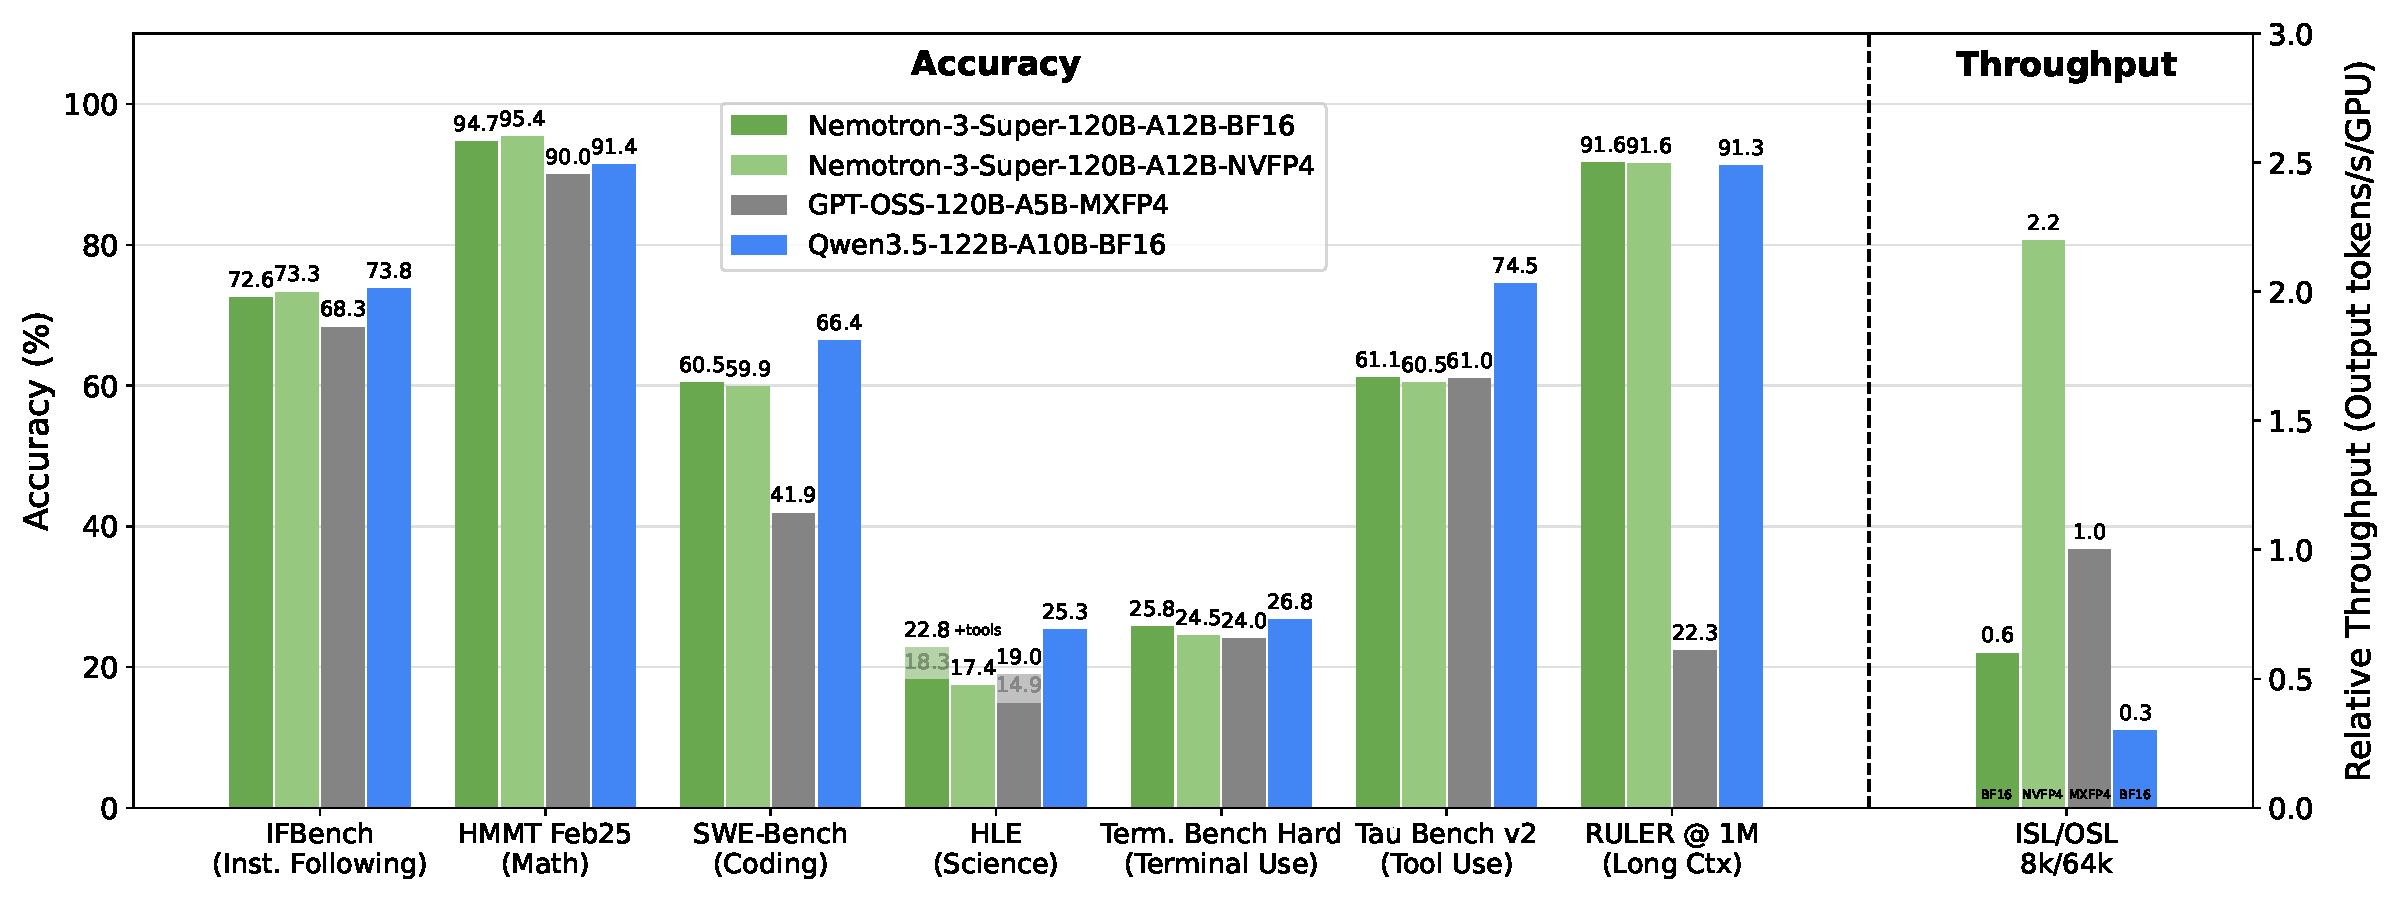
\includegraphics[width=\linewidth]{figures/superv3.pdf}
    \caption{Accuracy and throughput comparisons of \ourmodel with GPT-OSS-120B and Qwen3.5-122B. \ourmodel achieves comparable accuracies across popular benchmarks but provides the highest inference throughput; on 8k input sequence lengths and 64k output sequence lengths, \ourmodel provides up to 2.2$\times$ and 7.5$\times$ higher throughput than GPT-OSS-120B and Qwen3.5-122B, respectively. We measured throughput on B200 GPUs with vLLM and TRT-LLM and use the best out of the two frameworks for each model. For GPT-OSS-120B we use MXFP4 weights, MXFP8 activations, and FP8 KV-Cache; for Qwen3.5-122B we use BF16. We used the OpenHands harness to evaluate SWE-Bench.}
    \label{fig:intro}
\end{figure}

\ourmodel is our first model to use LatentMoE~\citep{latentmoe_tr} - a novel MoE architecture that achieves better accuracy per parameter and per FLOP than regular MoEs. \ourmodel also incorporates Multi-Token-Prediction (MTP), which accelerates inference through speculative decoding while improving overall model quality. We pre-trained \ourmodel in NVFP4, demonstrating stable and accurate pre-training in low precision. Similar to Nemotron 3 Nano~\citep{nvidia2025nemotron3nanoopen}, we pre-trained \ourmodel on 25 trillion text tokens divided into 2 phases. The first phase accounted for 80\% of pre-training (20 trillion tokens) and focused on diversity and broad coverage, while the second phase accounted for 20\% of pre-training (5 trillion tokens) and focused on high-quality data and benchmark accuracy. Our base model achieves significantly better accuracy than similarly sized state-of-the-art base models, such as GLM-4.5-Air-Base~\citep{5team2025glm45agenticreasoningcoding} and Ling-flash-Base-2.0~\citep{lingteam2025every}. 

We trained \ourmodel with a strong emphasis on agentic capabilities. To support this objective, we substantially scaled the breadth of our RL environments, the volume and quality of agentic training data, and the overall amount of post-training focused on multi-step tool-using behavior. To train effectively on this diverse set of long-horizon tasks, we made substantial improvements to the resiliency of our RL infrastructure, enabling large-scale asynchronous training. This expanded agentic training recipe yields substantial improvements over Nemotron 3 Nano across software engineering, terminal use, and general tool use benchmarks.

We are publicly sharing the training recipe for \ourmodel on the Nemotron Developer Repository\footnote{\href{https://github.com/NVIDIA-NeMo/Nemotron}{https://github.com/NVIDIA-NeMo/Nemotron}}. We are also openly releasing the following:

\newparagraph{Checkpoints}
\begin{itemize}
    \item \href{https://huggingface.co/nvidia/NVIDIA-Nemotron-3-Super-120B-A12B-NVFP4}{\texttt{Nemotron 3 Super 120B-A12B NVFP4} 
\includegraphics[height=0.9em]{assets/huggingface-color.png}} : post-trained and NVFP4 quantized model
    \item \href{https://huggingface.co/nvidia/NVIDIA-Nemotron-3-Super-120B-A12B-FP8}{\texttt{Nemotron 3 Super 120B-A12B FP8} 
\includegraphics[height=0.9em]{assets/huggingface-color.png}} : post-trained and FP8 quantized model
    \item \href{https://huggingface.co/nvidia/NVIDIA-Nemotron-3-Super-120B-A12B-BF16}{\texttt{Nemotron 3 Super 120B-A12B BF16} 
\includegraphics[height=0.9em]{assets/huggingface-color.png}} : post-trained model
    \item \href{https://huggingface.co/nvidia/NVIDIA-Nemotron-3-Super-120B-A12B-Base-BF16}{\texttt{Nemotron 3 Super 120B-A12B Base BF16} 
\includegraphics[height=0.9em]{assets/huggingface-color.png}} : base model
    \item \href{https://huggingface.co/nvidia/Qwen3-Nemotron-235B-A22B-GenRM-2603}{\texttt{Qwen3-Nemotron-235B-A22B-GenRM-2603} 
\includegraphics[height=0.9em]{assets/huggingface-color.png}} : GenRM used for RLHF
\end{itemize}


\newparagraph{Data}
\begin{itemize}
    \item \href{https://huggingface.co/datasets/nvidia/Nemotron-Pretraining-Specialized-v1.1}{\texttt{Nemotron-Pretraining-Specialized-v1.1} 
\includegraphics[height=0.9em]{assets/huggingface-color.png}} : a collection of synthetic datasets aimed to improve LLM capabilities in code concepts and algorithms, formal logic, economics, and multiple choice questions.
    \item \href{https://huggingface.co/collections/nvidia/nemotron-post-training-v3}{\texttt{Nemotron-Super-Post-Training-Data} } 
\includegraphics[height=0.9em]{assets/huggingface-color.png} : a collection of RL environments and SFT datasets targeting a broad range of agentic capabilities.
\end{itemize}

The report is organized into 3 broad sections: Pre-training~(\S\ref{sec:pretraining}), Post-training~(\S\ref{sec:alignment}), and Quantization~(\S\ref{sec:quantization}), each describing in detail our approach.

% 